\section{Технический проект}
\subsection{Общая характеристика организации решения задачи}

Полное наименование системы: кроссплатформенная программная система подбора попутчиков для автомобильных поездок.

Разрабатываемая программная система представляет собой платформу, позволяющую пользователям находить попутчиков для созданных автомобильных поездок. Данная система построена на клиент-серверной архитектуре.

Сервер – backend-модуль[{21}][{11}][{31}], обрабатывающий запросы клиентов. Сервер в данной программной системе один.

Функции, выполняемые на стороне сервера:

\begin{itemize}
	\item хранение, защита и доступ к данным;
	\item обработка поступающих клиентских запросов;
	\item поддержание целостности и актуальности данных;
	\item формирование и отправка ответов клиентам.
\end{itemize}

Одним из основных компонентов системы является база данных. В ней хранится практически вся информация, необходимая для работы системы, от данных пользователей до информации о предлагаемых и запрашиваемых поездках, а так же сведения об автомобилях, мессенджер, отзывы и рейтинг.

Задачи разработки включают:

\begin{itemize}
	\item проектирование и создание базы данных;
	\item разработка фонового сервиса для поддержания актуальности данных о поездках;
	\item проектирование и создание моделей данных;
	\item разработку контроллеров для обработки запросов;
	\item реализацию функционала для взаимодействия с базой данных.
\end{itemize}

\subsection{Обоснование выбора технологий проектирования}

Используемые для создания программно-информационной системы
языки и технологии отвечают современным практикам разработки, позволяют достичь высокой производительности и отказоустойчивости программы.

\subsubsection{Язык программирования C\#}

C\#[{1}][{2}][{3}] является одним из наиболее популярных и мощных языков программирования, который был разработан корпорацией Microsoft в рамках платформы .NET[{5}][{6}][{7}][{8}]. Одним из основных преимуществ C\# является его современный синтаксис, который сочетает в себе простоту и выразительность, что делает его удобным для изучения и использования как начинающими, так и опытными программистами. Этот язык позволяет разработчикам писать чистый, понятный и поддерживаемый код, что особенно важно при создании крупных и сложных приложений.

Еще одной значимой чертой C\# является его поддержка объектно-ориентированного программирования (ООП){[22]}{[23]}{[24]}. Это позволяет разработчикам создавать приложения, основываясь на принципах инкапсуляции, наследования и полиморфизма, что способствует созданию гибких и масштабируемых программных решений. ООП также облегчает повторное использование кода, что снижает затраты на разработку и поддержку программного обеспечения.

Богатый набор библиотек и инструментов, доступных для C\#, существенно упрощает разработку программ. Эти библиотеки покрывают широкий спектр задач — от работы с базами данных и сетевыми взаимодействиями до создания пользовательских интерфейсов и работы с файлами. Благодаря этому разработчики могут сосредоточиться на решении бизнес-задач, не тратя много времени на создание базовой функциональности с нуля.

Среда разработки Visual Studio[{9}][{10}][{13}][{14}], в которой часто ведется разработка на C\#, предлагает мощные средства для написания, отладки и тестирования кода. Интегрированные средства автоматизации, рефакторинга и анализа кода помогают разработчикам повышать продуктивность и качество конечного продукта. Это позволяет быстро находить и исправлять ошибки, а также оптимизировать код для повышения его производительности.

C\# также обладает высокой безопасностью типов, что предотвращает многие распространенные ошибки, такие как доступ к неинициализированным переменным или некорректное приведение типов. Управление памятью в C\# осуществляется с помощью сборщика мусора, что упрощает процесс управления ресурсами и снижает вероятность утечек памяти.

Кроме того, сообщество разработчиков C\# активно и постоянно растет, предоставляя богатый выбор ресурсов для обучения и обмена опытом. Это включает в себя форумы, блоги, видеоуроки и другие формы поддержки, которые помогают разработчикам быстро находить ответы на возникающие вопросы и постоянно совершенствовать свои навыки.

Таким образом, выбор C\# в качестве языка программирования предоставляет разработчикам мощные инструменты для создания современных, эффективных и надежных приложений, что делает его отличным выбором для самых разнообразных проектов.

\subsubsection{Фреймворк ASP.net}

ASP.NET[{15}][{16}][{17}][{18}] — это мощная и гибкая платформа для разработки веб-приложений, созданная корпорацией Microsoft. Один из основных факторов, делающих ASP.NET привлекательным выбором для разработчиков, — это его интеграция с экосистемой .NET. Это позволяет использовать все возможности языка программирования C\#, а также широкий набор библиотек и инструментов, что существенно ускоряет процесс разработки и упрощает создание высокопроизводительных и масштабируемых веб-приложений.

ASP.NET предоставляет разработчикам множество возможностей для создания динамических веб-страниц и приложений. Он поддерживает модель программирования, которая включает в себя серверные элементы управления, такие как формы и сетки данных, что позволяет создавать интерактивные и отзывчивые пользовательские интерфейсы с минимальными усилиями. Это особенно важно для создания сложных веб-приложений, которые требуют высокого уровня интерактивности и пользовательского опыта.

Одним из ключевых преимуществ ASP.NET является его высокая производительность. Платформа оптимизирована для обработки больших объемов запросов и может эффективно управлять ресурсами, что позволяет создавать быстрые и отзывчивые веб-приложения. ASP.NET также поддерживает асинхронное программирование, что улучшает масштабируемость приложений и снижает нагрузку на серверы.

Безопасность является еще одной важной чертой ASP.NET. Платформа предоставляет встроенные механизмы защиты от распространенных угроз веб-безопасности, таких как межсайтовый скриптинг (XSS)[{19}][{20}], SQL-инъекции[{25}][{26}]и другие виды атак. Это позволяет разработчикам сосредоточиться на функциональности приложений, не беспокоясь о внедрении сложных мер безопасности.

ASP.NET также поддерживает модульность и повторное использование кода. Это достигается благодаря компонентам, таким как контроллеры и представления в ASP.NET MVC[{27}][{28}][{29}][{32}], которые могут быть легко переработаны и использованы в различных частях приложения. Это способствует более эффективной разработке и снижает затраты на поддержку кода.

Кроме того, сообщество разработчиков ASP.NET активно и постоянно растет. Это обеспечивает обширную базу знаний и ресурсов, доступных для обучения и обмена опытом. Форумы, блоги, документация и видеоуроки помогают разработчикам быстро находить решения для возникающих проблем и улучшать свои навыки.

Таким образом, выбор ASP.NET в качестве платформы для разработки веб-приложений предоставляет разработчикам мощные инструменты и возможности для создания надежных, безопасных и высокопроизводительных веб-приложений. Платформа сочетает в себе современные технологии и подходы, что делает её отличным выбором для самых разнообразных проектов, от небольших сайтов до крупных корпоративных приложений.

\subsubsection{Расширение T-SQL}

T-SQL (Transact-SQL) — это расширение стандартного языка SQL (Structured Query Language), разработанное корпорацией Microsoft для управления и манипулирования данными в реляционных базах данных, таких как Microsoft SQL Server. Одной из ключевых причин выбора T-SQL{[30]}{[33]} является его тесная интеграция с Microsoft SQL Server{[34]}{[35]}, что делает его мощным инструментом для разработки сложных запросов, процедур и скриптов, необходимых для управления данными и обеспечения их целостности.

Одним из значимых преимуществ T-SQL является его расширенные возможности по сравнению с обычным SQL. T-SQL включает в себя дополнительные конструкции, такие как циклы, условные операторы и встроенные функции, что позволяет разработчикам создавать более сложные и функциональные запросы. Это особенно важно для выполнения сложных бизнес-логик и операций с данными, которые требуют более гибких и мощных инструментов.

T-SQL также поддерживает создание хранимых процедур, триггеров и пользовательских функций. Хранимые процедуры позволяют выполнять сложные операции над данными, объединяя несколько SQL-запросов в один логический блок, что упрощает управление кодом и повышает его повторное использование. Триггеры позволяют автоматически выполнять определенные действия при изменении данных в таблице, что помогает поддерживать целостность данных и автоматизировать рутинные задачи.

Еще одной важной чертой T-SQL является его мощные средства для обработки и анализа данных. T-SQL предоставляет широкий набор функций для работы с текстом, датами, числами и другими типами данных, что облегчает выполнение различных операций над данными. Кроме того, T-SQL поддерживает создание временных таблиц и курсоров, что позволяет разработчикам эффективно управлять временными данными и выполнять сложные операции над ними.

Производительность также является важным аспектом T-SQL. Разработчики могут оптимизировать запросы с помощью индексов, оптимизатора запросов и других инструментов, что позволяет значительно повысить скорость выполнения операций над данными. Это особенно важно для работы с большими объемами данных, где производительность имеет критическое значение.

T-SQL также обеспечивает высокую степень безопасности данных. Разработчики могут использовать механизмы управления правами доступа, чтобы контролировать, кто и какие операции может выполнять над данными. Это помогает защитить данные от несанкционированного доступа и обеспечивать их конфиденциальность и целостность.

Кроме того, сообщество разработчиков T-SQL активно и постоянно растет, что обеспечивает широкий доступ к ресурсам для обучения и обмена опытом. Форумы, блоги, документация и видеоуроки помогают разработчикам быстро находить ответы на возникающие вопросы и совершенствовать свои навыки.

Таким образом, выбор T-SQL в качестве языка для работы с базами данных предоставляет разработчикам мощные и гибкие инструменты для управления данными, выполнения сложных операций и обеспечения их целостности и безопасности. Это делает T-SQL отличным выбором для разработки и поддержки надежных и эффективных решений для управления данными в корпоративных и других приложениях.

\subsubsection{Протокол связи HTTP}

HTTP (Hypertext Transfer Protocol) — это основополагающий протокол для передачи данных в интернете, который служит базой для обмена информацией между веб-серверами и клиентами, такими как браузеры. Протокол был разработан в начале 1990-х годов в Европейской организации по ядерным исследованиям (CERN) под руководством Тима Бернерса-Ли и Роберта Кайо, и с тех пор HTTP{[36]}{[37]} стал стандартом для передачи гипертекстовых документов в сети.

Одним из ключевых аспектов HTTP является его простота и универсальность. HTTP использует текстовый формат для передачи данных, что делает его легко читаемым и понятным как для машин, так и для людей. Запросы и ответы в HTTP формируются в виде строк, что упрощает процесс их анализа и отладки. Клиент (обычно браузер) отправляет запрос серверу, который обрабатывает его и возвращает ответ, содержащий запрашиваемые данные, статус выполнения запроса и метаинформацию.

HTTP — это протокол уровня приложения, который работает поверх других протоколов, таких как TCP/IP{[38]}{[39]}. Это позволяет ему обеспечивать надежную и последовательную доставку данных, а также корректировать ошибки передачи. HTTP поддерживает широкий спектр методов, каждый из которых предназначен для выполнения определенных действий. Наиболее распространенные из них — GET, POST, PUT и DELETE. Метод GET используется для запроса данных с сервера, POST — для отправки данных на сервер, PUT — для обновления существующих данных, а DELETE — для удаления данных.

Преимущество HTTP в его гибкости и способности адаптироваться под различные нужды. Например, современные веб-приложения используют HTTP для взаимодействия с API, что позволяет обмениваться данными между различными системами и сервисами. HTTP также поддерживает работу с мультимедийным контентом, таким как изображения, видео и аудио, что делает его идеальным для создания разнообразных веб-приложений.

Безопасность передачи данных является важным аспектом HTTP. Для обеспечения конфиденциальности и целостности данных используется протокол HTTPS, который представляет собой HTTP, работающий поверх SSL/TLS. HTTPS обеспечивает шифрование данных, передаваемых между клиентом и сервером, что защищает их от перехвата и изменения злоумышленниками. В наши дни использование HTTPS стало стандартом для большинства веб-сайтов, особенно тех, которые обрабатывают конфиденциальную информацию, такую как личные данные или данные кредитных карт.

Кроме того, HTTP поддерживает кэширование, что позволяет сохранять копии веб-страниц и других ресурсов для ускорения их загрузки при повторных обращениях. Это существенно улучшает пользовательский опыт, так как сокращает время ожидания и уменьшает нагрузку на серверы. Также HTTP поддерживает возможность сжатия данных, что снижает объем передаваемых данных и ускоряет их доставку.

HTTP продолжает развиваться, предлагая новые возможности и улучшения, которые позволяют разрабатывать более эффективные, безопасные и производительные веб-приложения. Независимо от сложности и масштабов проекта, HTTP остается фундаментальным инструментом для передачи данных в интернете.

\subsection{Проект данных программной системы}

На основании анализа предметной области из технического задания была разработана база данных.

База данных включает в себя следующие таблицы:

\begin{enumerate}
	\item Users - пользователи системы.
	\item Cars - пользовательские автомобили.
	\item Passengers - пассажиры забронировавшие поездку.
	\item Travels - поездки созданные водителем.
	\item DriverTravel - таблица связи, необходимая для привязки водителя и поездки.
	\item Chats - пользовательские чаты.
	\item Messages - сообщения в чате.
	\item Comments - комментарии под профилем.
\end{enumerate}

На рисунке 3.1 изображена ER-диаграмма базы данных.

\begin{figure}[H]
	\centering
	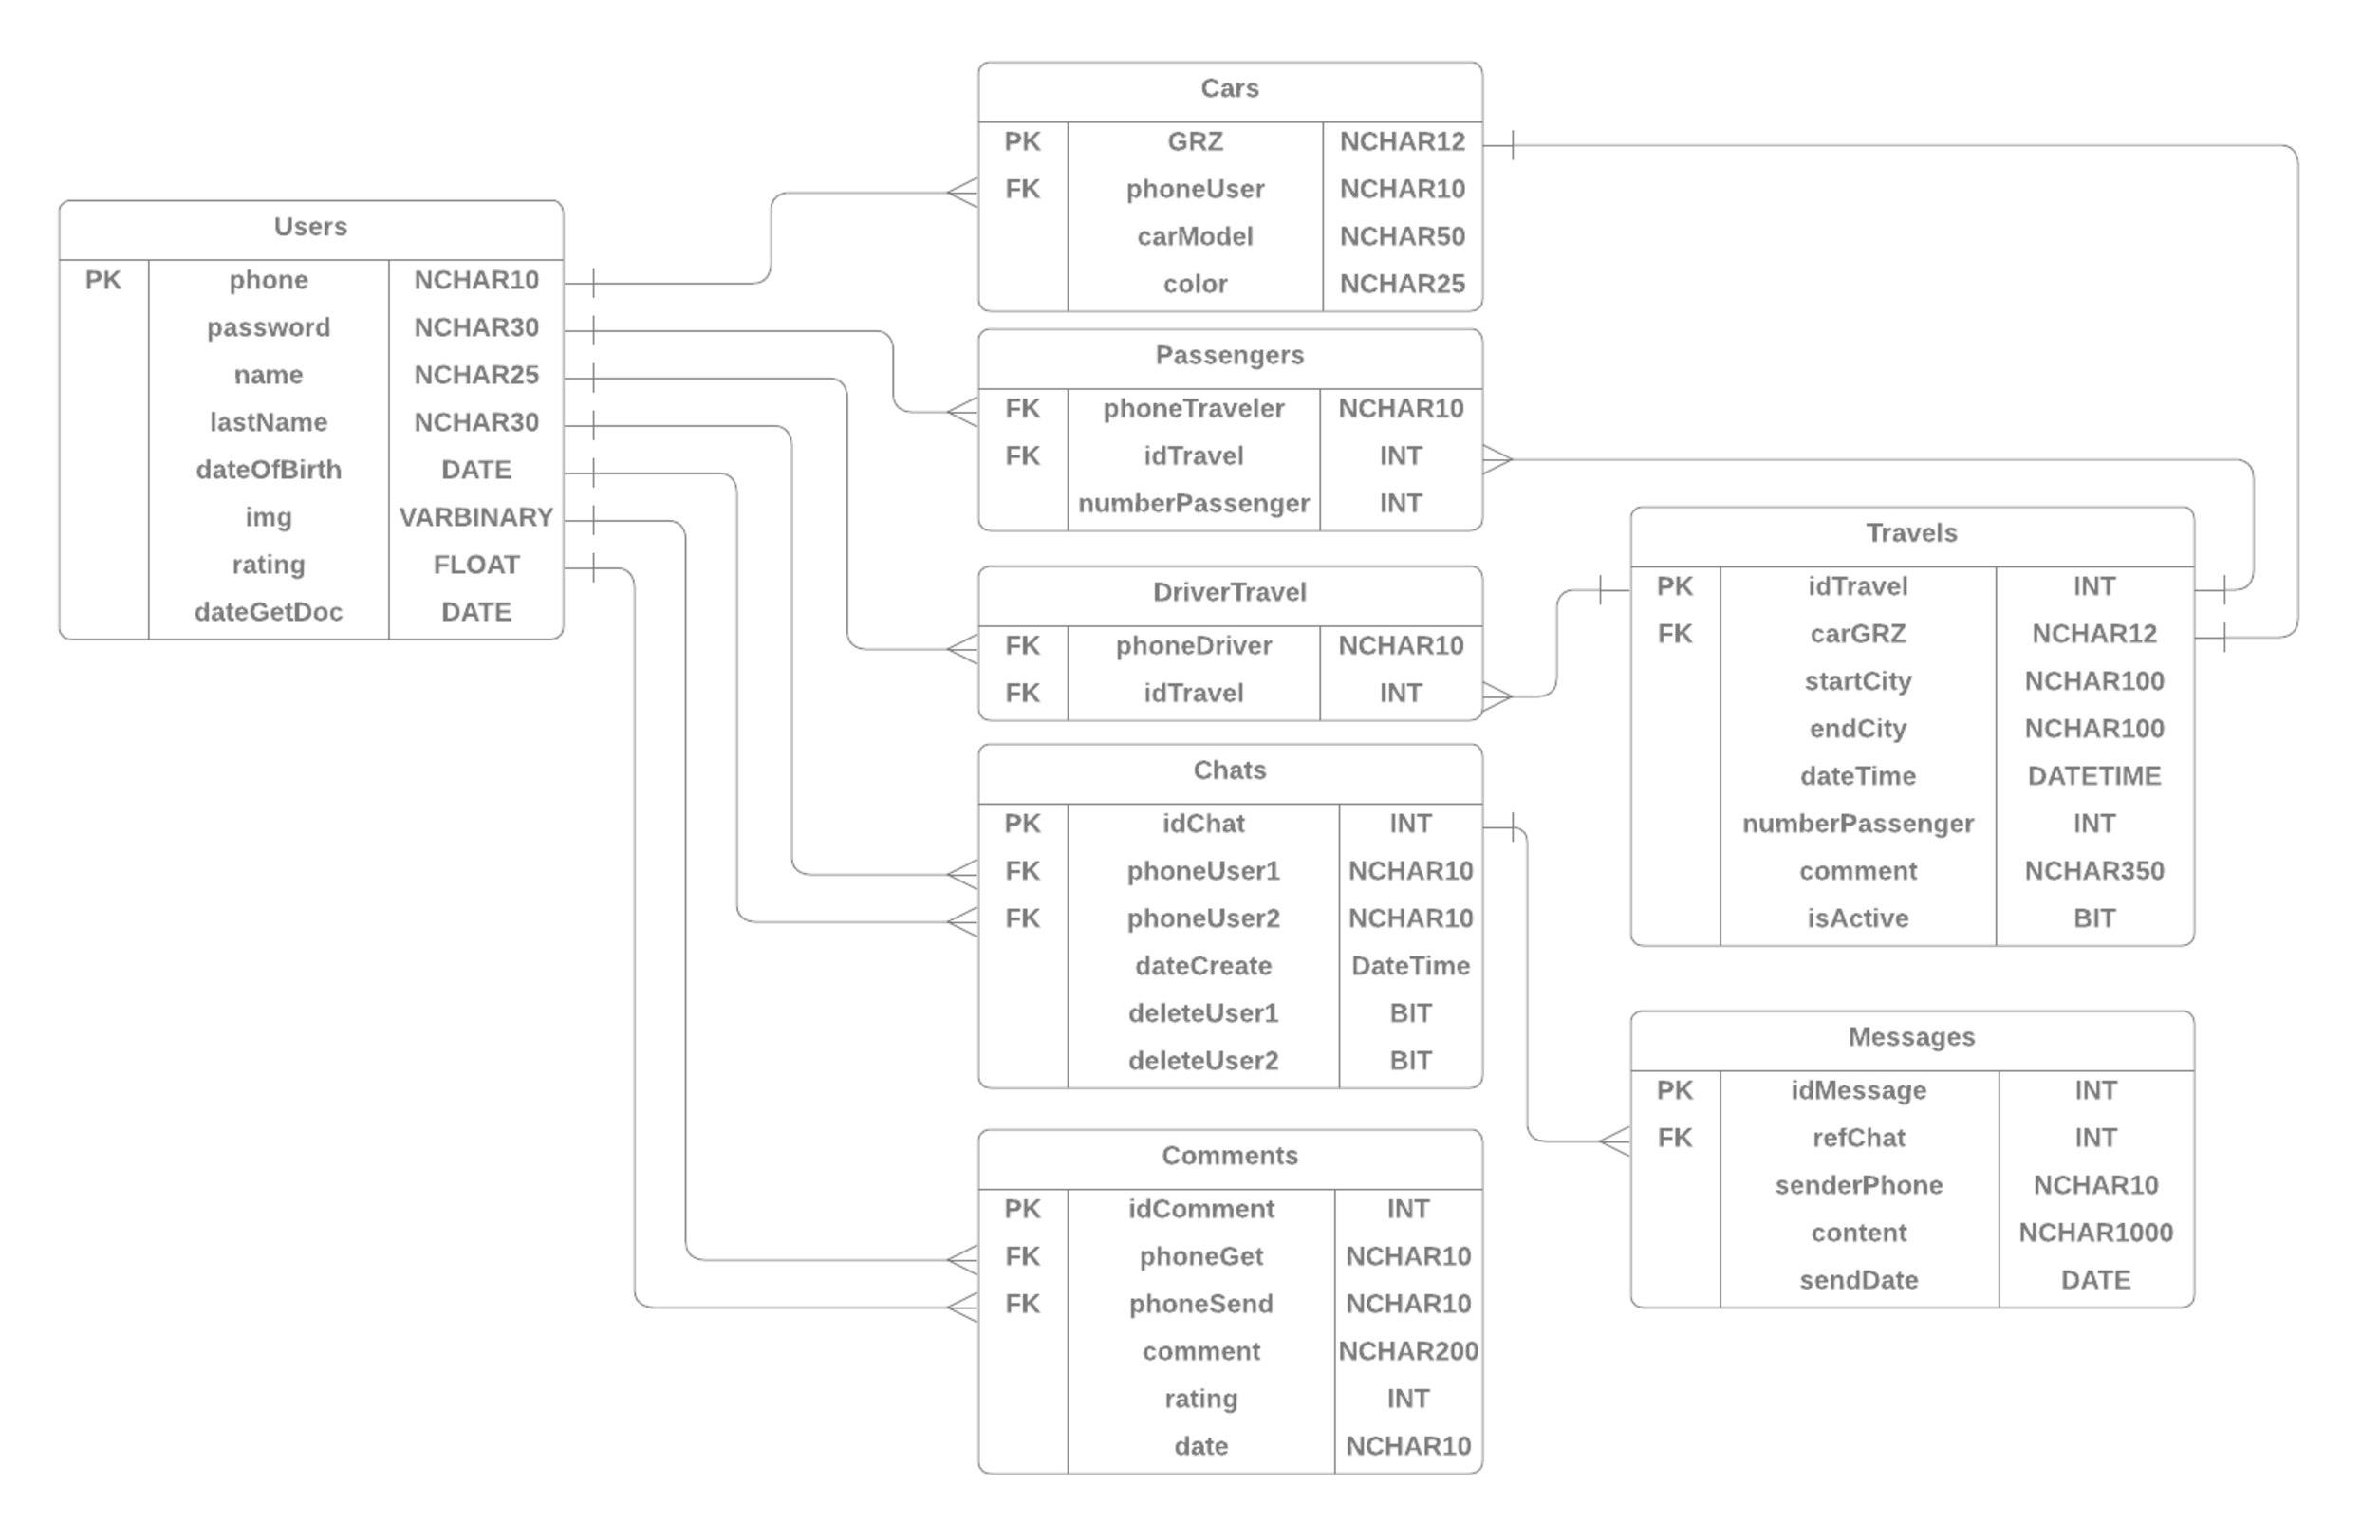
\includegraphics[width=0.9\linewidth]{images/ErDiagramDB}
	\caption{ER-диаграмма базы данных}
	\label{fig:erdiagramdb}
\end{figure}

В таблицах 3.1-3.8 представлены атрибуты таблиц базы данных.

\begin{xltabular}{\textwidth}{|X|X|X|}
	\caption{Атрибуты таблицы Users\label{ssevsws:table}}\\ \hline
	\centrow Название атрибута & \centrow Тип данных & \centrow Описание \\ \hline
	\endfirsthead
	\continuecaption{Продолжение таблицы \ref{ssevsws:table}}
	\centrow Название атрибута & \centrow Тип данных & \centrow Описание \\ \hline 
	\finishhead
	phone & NVARCHAR(10) & Номер телефона пользователя\\ \hline 
	password & NVARCHAR(30) & Пароль от учетной записи \\ \hline 
	name & NVARCHAR(25) & Имя пользователя \\ \hline 
	lastName & NVARCHAR(30) & Фамилия пользователя \\ \hline
	dateOfBirth & DATE & Дата рождения \\ \hline
	img & VARBINARY(MAX) & Фотография пользователя \\ \hline 
	rating & FLOAT & Рейтинг \\ \hline 
	dateGetDoc & DATE & Дата получения водительского удостоверения \\ \hline 
\end{xltabular}

\begin{xltabular}{\textwidth}{|X|X|X|}
	\caption{Атрибуты таблицы Cars\label{ssevsws:table}}\\ \hline
	\centrow Название атрибута & \centrow Тип данных & \centrow Описание \\ \hline
	\endfirsthead
	\continuecaption{Продолжение таблицы \ref{ssevsws:table}}
	\centrow Название атрибута & \centrow Тип данных & \centrow Описание \\ \hline 
	\finishhead
	GRZ & NVARCHAR(12) & Государственный регистрационный знак автомобиля \\ \hline 
	phoneUser & NVARCHAR(10) & FK на номер телефона \\ \hline 
	carModel & NVARCHAR(50) & Модель автомобиля \\ \hline 
	color & NVARCHAR(25) & Цвет автомобиля \\ \hline 
\end{xltabular}

\begin{xltabular}{\textwidth}{|X|X|X|}
	\caption{Атрибуты таблицы Passengers\label{ssevsws:table}}\\ \hline
	\centrow Название атрибута & \centrow Тип данных & \centrow Описание \\ \hline
	\endfirsthead
	\continuecaption{Продолжение таблицы \ref{ssevsws:table}}
	\centrow Название атрибута & \centrow Тип данных & \centrow Описание \\ \hline 
	\finishhead
	phoneTraveler & NVARCHAR(10) & FK на номер телефона попутчика \\ \hline 
	idTravel & INT & FK на уникальный идентификатор поездки \\ \hline 
	numberPassenger & INT & Количество пассажиров \\ \hline  
\end{xltabular}

\begin{xltabular}{\textwidth}{|X|X|X|}
	\caption{Атрибуты таблицы Travels\label{tb}}\\ \hline
	\centrow Название атрибута & \centrow Тип данных & \centrow Описание \\ \hline
	\endfirsthead
	\continuecaption{Продолжение таблицы \ref{tb}}
	\centrow Название атрибута & \centrow Тип данных & \centrow Описание \\ \hline 
	\finishhead
	idTravel & INT & Уникальнаый идентификатор поездки \\ \hline 
	carGRZ & NVARCHAR(12) & FK на ГРЗ автомобиля \\ \hline 
	startCity & NVARCHAR(100) & Город начала маршрута \\ \hline
	endCity & NVARCHAR(100) & Город окончания маршрута \\ \hline
	dateTime & DATETIME & Дата и время поездки \\ \hline
	numberPassenger & INT & Количество пассажиров в поездке \\ \hline
	comment & NVARCHAR(350) & Комментарий к поездке \\ \hline
	isActive & BIT & Статус активности \\ \hline  
\end{xltabular}

\begin{xltabular}{\textwidth}{|X|X|X|}
	\caption{Атрибуты таблицы DriverTravel\label{ssevsws:table}}\\ \hline
	\centrow Название атрибута & \centrow Тип данных & \centrow Описание \\ \hline
	\endfirsthead
	\continuecaption{Продолжение таблицы \ref{ssevsws:table}}
	\centrow Название атрибута & \centrow Тип данных & \centrow Описание \\ \hline 
	\finishhead
	phoneDriver & NVARCHAR(10) & FK на номер телефона водителя \\ \hline 
	idTravel & INT & FK на уникальный идентификатор поездки \\ \hline 
\end{xltabular}

\begin{xltabular}{\textwidth}{|X|X|X|}
	\caption{Атрибуты таблицы Chats\label{ssevsws:table}}\\ \hline
	\centrow Название атрибута & \centrow Тип данных & \centrow Описание \\ \hline
	\endfirsthead
	\continuecaption{Продолжение таблицы \ref{ssevsws:table}}
	\centrow Название атрибута & \centrow Тип данных & \centrow Описание \\ \hline 
	\finishhead
	idChat & INT & Уникальный идентификатор чата \\ \hline 
	phoneUser1 & NVARCHAR(10) & FK на номер телефона \\ \hline 
	phoneUser2 & NVARCHAR(10) & FK на номер телефона \\ \hline
	dateCreate & DateTime & Дата и время создания чата \\ \hline
	deleteUser1 & BIT & Статус удаленного чата у первого собесденика \\ \hline
	deleteUser2 & BIT & Статус удаленного чата у второго собесденика \\ \hline
\end{xltabular}

\begin{xltabular}{\textwidth}{|X|X|X|}
	\caption{Атрибуты таблицы Messages\label{ssevsws:table}}\\ \hline
	\centrow Название атрибута & \centrow Тип данных & \centrow Описание \\ \hline
	\endfirsthead
	\continuecaption{Продолжение таблицы \ref{ssevsws:table}}
	\centrow Название атрибута & \centrow Тип данных & \centrow Описание \\ \hline 
	\finishhead
	idMessage & INT & Уникальный идентификатор сообщения \\ \hline 
	refChat & INT & FK на чат \\ \hline 
	senderPhone & NVARCHAR(10) & Номер телефона отправителя \\ \hline
	content & NVARCHAR(1000) & Текст сообщения \\ \hline
	sendDate & DateTime & дата и время отправки \\ \hline
\end{xltabular}

\begin{xltabular}{\textwidth}{|X|X|X|}
	\caption{Атрибуты таблицы Comments\label{ssevsws:table}}\\ \hline
	\centrow Название атрибута & \centrow Тип данных & \centrow Описание \\ \hline
	\endfirsthead
	\continuecaption{Продолжение таблицы \ref{ssevsws:table}}
	\centrow Название атрибута & \centrow Тип данных & \centrow Описание \\ \hline 
	\finishhead
	idComment & INT & Уникальный идентификатор комментария \\ \hline 
	phoneGet & NVARCHAR(10) & Телефон получателя \\ \hline 
	phoneSend & NVARCHAR(10) & Телефон отправителя \\ \hline
	comment & NVARCHAR(200) & Текст комментария \\ \hline
	rating & INT & Оценка \\ \hline
	date & DATE & Дата комментария \\ \hline 
\end{xltabular}

\subsection{Проектирование архитектуры программной системы}
\subsubsection{Компоненты программной системы}

Разрабатываемая система представляет из себя серверное приложение.
Для разработки backend-модуля будет использоваться язык программирования C\# 10.0{[40]} с применением фреймворка ASP.Net для создания серверного модуля и фреймворка SqlClient{[39]} для обеспечения доступа к базе данных.

Используемая среда разработки – Visual Studio 2022.

В качестве СУБД необходимо использовать Microsoft SQL Server.

В качестве системы управления версиями для командной разработки необходимо использовать Git{[41]}{[42]}{[43]}.

Диаграмма развёртывания программы представлена на рисунке 3.2

\begin{figure}[H]
	\centering
	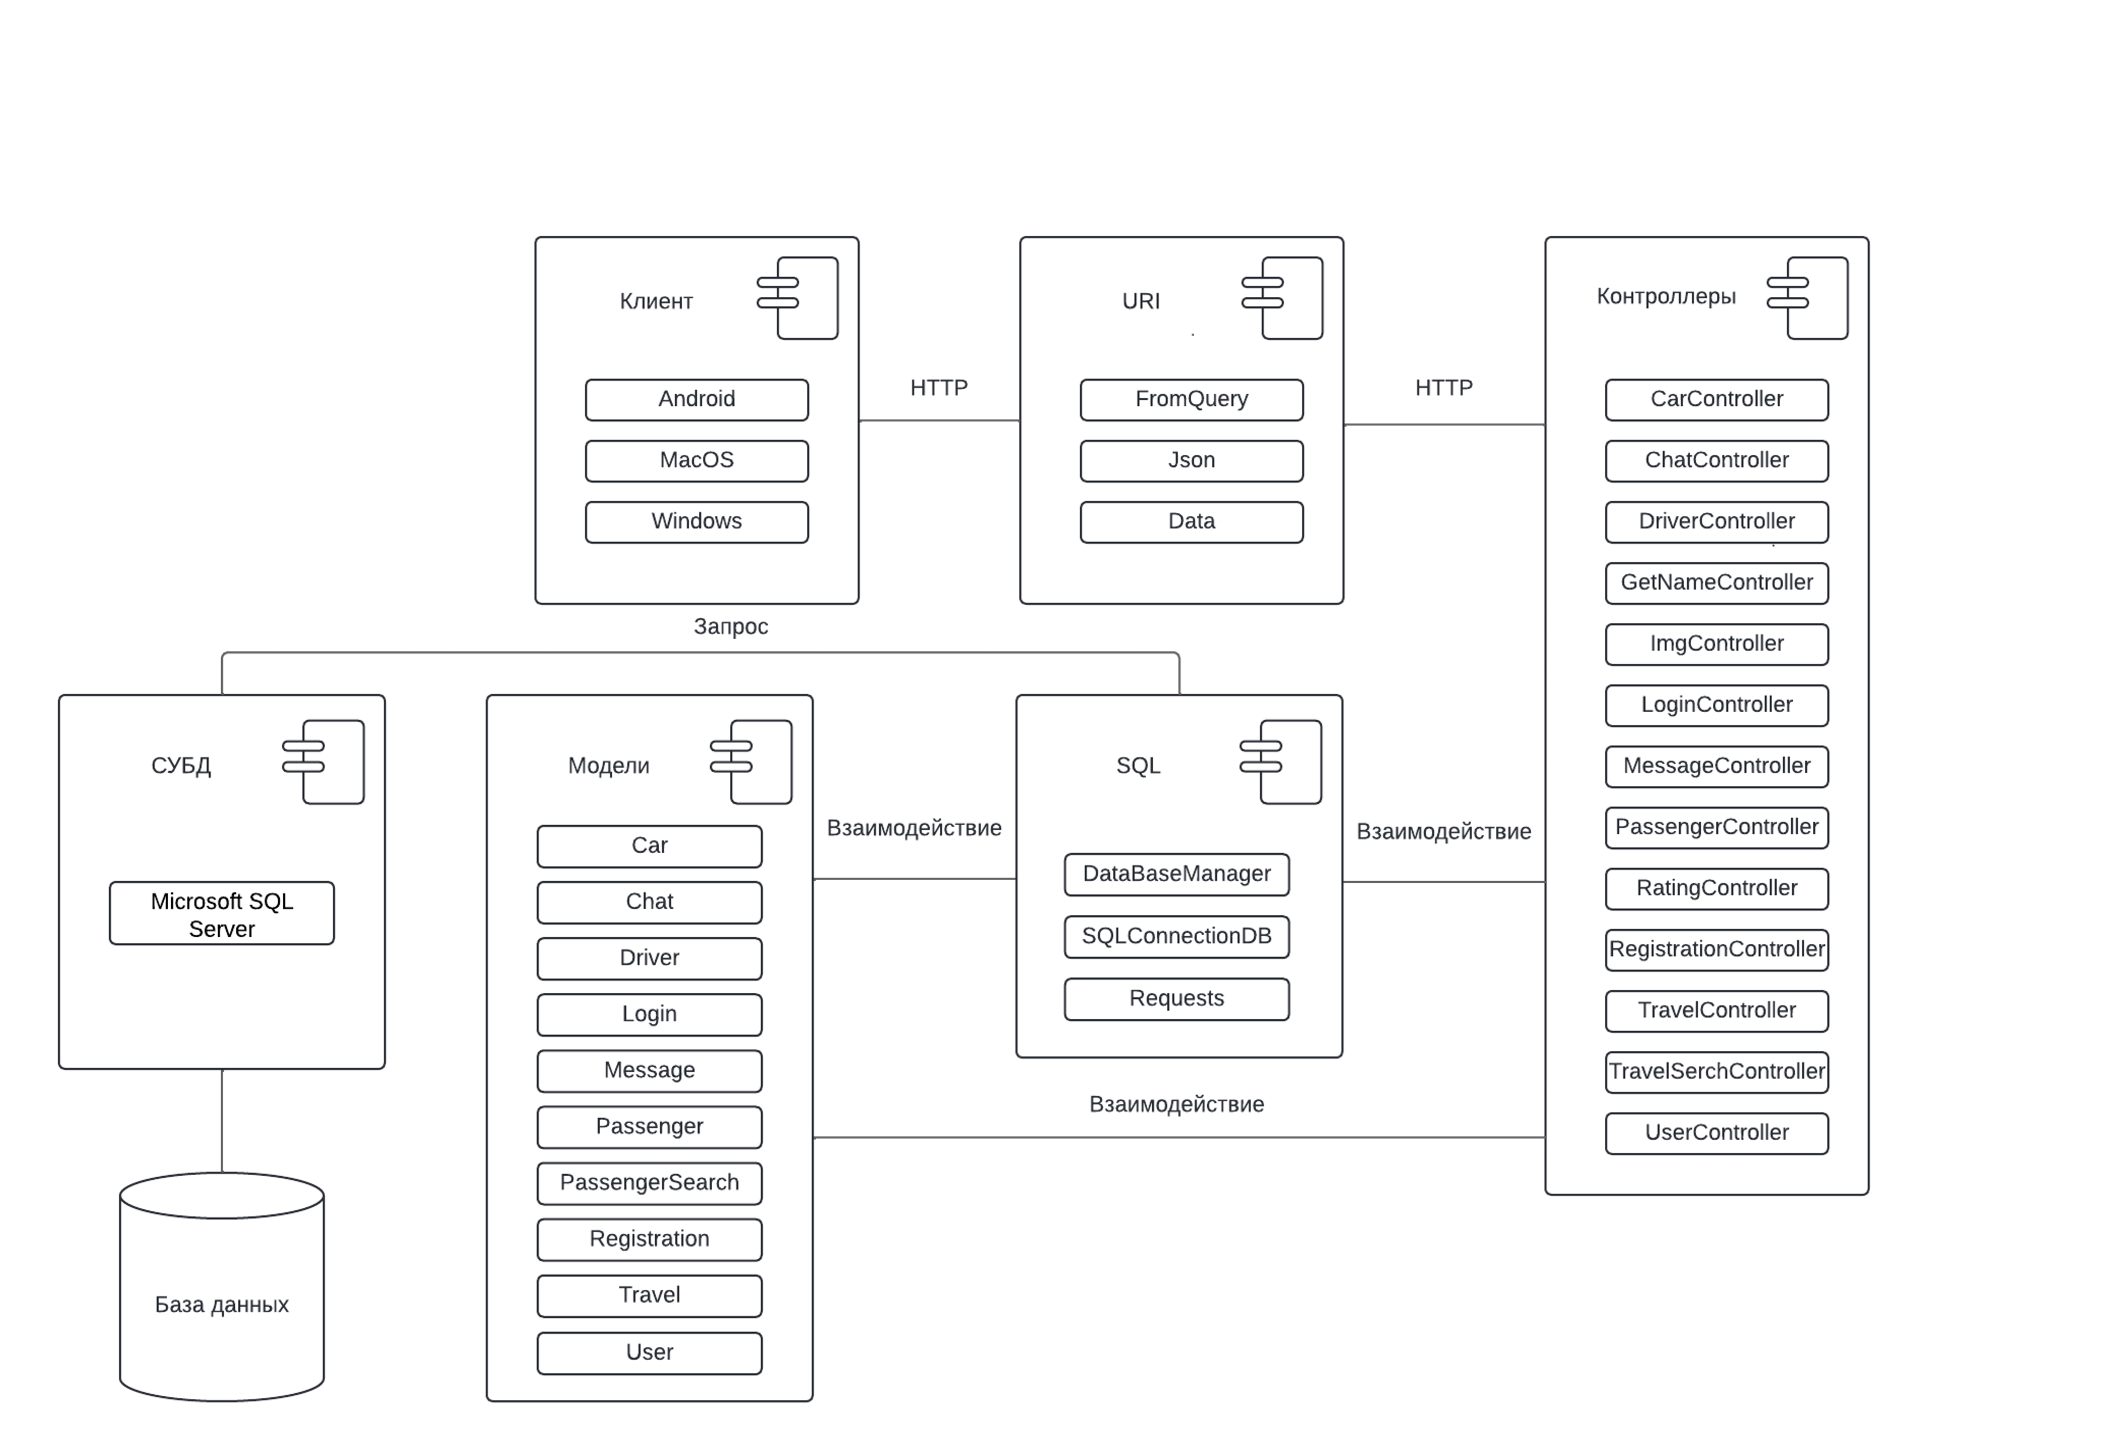
\includegraphics[width=0.9\linewidth]{images/diagramArch}
	\caption{Диаграмма развертывания программы}
	\label{fig:diagramarch}
\end{figure}

Программно-информационная система состоит из нескольких ключевых компонентов, каждый из которых выполняет свои уникальные функции, обеспечивая бесперебойную работу всей платформы. В центре этой системы находится клиентская часть, представленная приложениями для различных операционных систем, таких как Android, MacOS и Windows. Эти приложения позволяют пользователям взаимодействовать с системой через HTTP-запросы, обеспечивая доступ к необходимым функциям и данным.

Одним из важнейших компонентов системы является URI, который обрабатывает запросы, поступающие от клиентов. URI играет ключевую роль в маршрутизации и управлении данными, обрабатывая параметры запросов, работая с JSON-данными[{44}][{45}] и управляя передаваемыми данными. Благодаря этому компоненту, система может эффективно и безопасно обмениваться информацией между клиентами и серверами. URI, в свою очередь, направляет запросы к соответствующим контроллерам, которые отвечают за выполнение конкретных задач.

Контроллеры представляют собой еще один важный элемент системы. Они отвечают за выполнение различных операций, связанных с функциональностью системы. Контроллеры управляют данными о транспортных средствах, чатами между пользователями, информацией о водителях, а также процессами аутентификации и регистрации пользователей. Они также занимаются управлением сообщениями, пассажирами, рейтингами, поездками и данными пользователей, обеспечивая координацию и выполнение всех основных функций системы. Каждый запрос, поступающий от клиента через URI, направляется к соответствующему контроллеру для обработки и выполнения необходимых операций.

Модели представляют собой набор компонентов, которые описывают основные сущности системы. Они включают в себя такие важные элементы, как транспортные средства, чаты, водители, пассажиры, поездки и пользователи. Эти модели играют ключевую роль в взаимодействии с базой данных, обеспечивая структурированный и организованный подход к хранению и обработке данных. Взаимодействие моделей с базой данных осуществляется через слой SQL, который включает в себя управление базой данных, установление и управление соединениями, а также обработку запросов к базе данных. Контроллеры взаимодействуют с моделями для выполнения операций чтения и записи данных, обеспечивая тем самым актуальность и консистентность данных в системе.

СУБД, используемая в системе, представлена Microsoft SQL Server. Эта система управления базами данных обеспечивает надежное и эффективное хранение всех данных, необходимых для работы платформы. Взаимодействие с базой данных осуществляется через SQL-компоненты, что позволяет обеспечить высокую производительность и надежность при работе с большими объемами данных. Модели обращаются к SQL для выполнения операций с данными, таких как запросы, обновления и удаления, гарантируя, что все данные, хранящиеся в базе данных, актуальны и доступны для обработки.

Таким образом, программно-информационная система представляет собой сложную и многоуровневую структуру, включающую в себя клиентскую часть, URI, контроллеры, модели, слой SQL и СУБД. Взаимодействие между этими компонентами осуществляется через четко определенные интерфейсы и протоколы, обеспечивая функциональность, надежность и безопасность всей платформы. Клиентские приложения отправляют запросы через URI, который маршрутизирует их к соответствующим контроллерам. Контроллеры, в свою очередь, взаимодействуют с моделями и SQL для выполнения необходимых операций с данными. Все данные хранятся в надежной СУБД, обеспечивая целостность и доступность информации. Взаимодействие между этими компонентами позволяет системе эффективно выполнять свои задачи и обеспечивать пользователям доступ к необходимым данным и функциям.

\subsubsection{Архитектура программной системы}

Архитектура MVC (Model-View-Controller) является широко распространенной парадигмой проектирования программного обеспечения, которая способствует разделению приложения на три взаимосвязанных компонента: модель, представление и контроллер. Эта архитектура позволяет улучшить управляемость, модульность и тестируемость кода.

Модель (Model)

Модель отвечает за управление данными и бизнес-логикой приложения. Она представляет собой центральную часть архитектуры, где происходят все операции с данными. Модель определяет структуру данных, правила их обработки и взаимодействие с базами данных или другими источниками данных. В модели реализуются основные функции, такие как получение, сохранение, обновление и удаление данных. Модель также уведомляет представление о необходимости обновления данных, чтобы обеспечить синхронизацию между состоянием данных и их отображением.

Представление (View)

Представление отвечает за отображение данных пользователю. Оно получает данные от модели и отображает их в удобной и понятной форме. Представление не содержит логики обработки данных; его задача — только визуализация информации. В веб-приложениях это могут быть HTML-страницы, шаблоны или компоненты пользовательского интерфейса. Важно отметить, что представление не взаимодействует напрямую с моделью, а получает данные через контроллер, что способствует снижению зависимости между компонентами.

Контроллер (Controller)

Контроллер служит посредником между моделью и представлением. Он обрабатывает входные данные от пользователя, вызывает соответствующие методы модели для обработки этих данных и обновляет представление в соответствии с результатами работы модели. Контроллеры принимают запросы от пользователей, определяют, какие действия должны быть выполнены, и управляют потоком данных между моделью и представлением. Благодаря этому контроллеры обеспечивают логическую связь между компонентами системы и позволяют изолировать бизнес-логику от пользовательского интерфейса.

Взаимодействие между компонентами:

\begin{itemize}
	\item Модель и Представление. Модель обновляет данные и уведомляет представление о необходимости изменения отображения. Представление запрашивает данные у модели и обновляется в соответствии с изменениями.
	\item Модель и Контроллер. Контроллер взаимодействует с моделью для выполнения операций над данными. Он отправляет запросы модели на изменение данных и получает обновленные данные для последующей передачи представлению.
	\item Контроллер и Представление. Контроллер управляет отображением данных, передавая модели необходимые запросы и обновляя представление в соответствии с результатами работы модели. Контроллер обрабатывает пользовательские запросы и определяет, какие действия нужно предпринять, чтобы ответить на эти запросы.
\end{itemize}

Преимущества архитектуры MVC:

\begin{itemize}
	\item Разделение обязанностей. Разделение кода на три компонента улучшает управляемость и упрощает сопровождение приложения.
	\item Модульность. Каждый компонент можно разрабатывать и тестировать независимо от других, что ускоряет процесс разработки.
	\item Повышенная тестируемость. Благодаря четкому разделению обязанностей проще писать и выполнять автоматические тесты для каждого компонента.
	\item Масштабируемость. Архитектура MVC облегчает добавление новых функций и компонентов без значительного изменения существующего кода.
	\item Гибкость. Легче менять или обновлять отдельные компоненты системы, такие как пользовательский интерфейс, не затрагивая бизнес-логику.
\end{itemize}

Архитектура MVC, благодаря своему структурированному подходу и разделению обязанностей, помогает создавать более надежные, поддерживаемые и масштабируемые приложения.

\subsubsection{Архитектура программных классов моделей и контроллеров}

IActionResult - это интерфейс, который представляет результат действия в ASP.NET Core. Контроллеры возвращают объекты, реализующие этот интерфейс, чтобы сообщить о результате выполнения запроса. Например, это может быть возвращение данных, сообщение об ошибке или перенаправление.

На рисунке 3.3 представлена UML-диаграмма классов программной системы, отражающих взаимодействие моделей и контроллеров.

\begin{figure}[H]
	\centering
	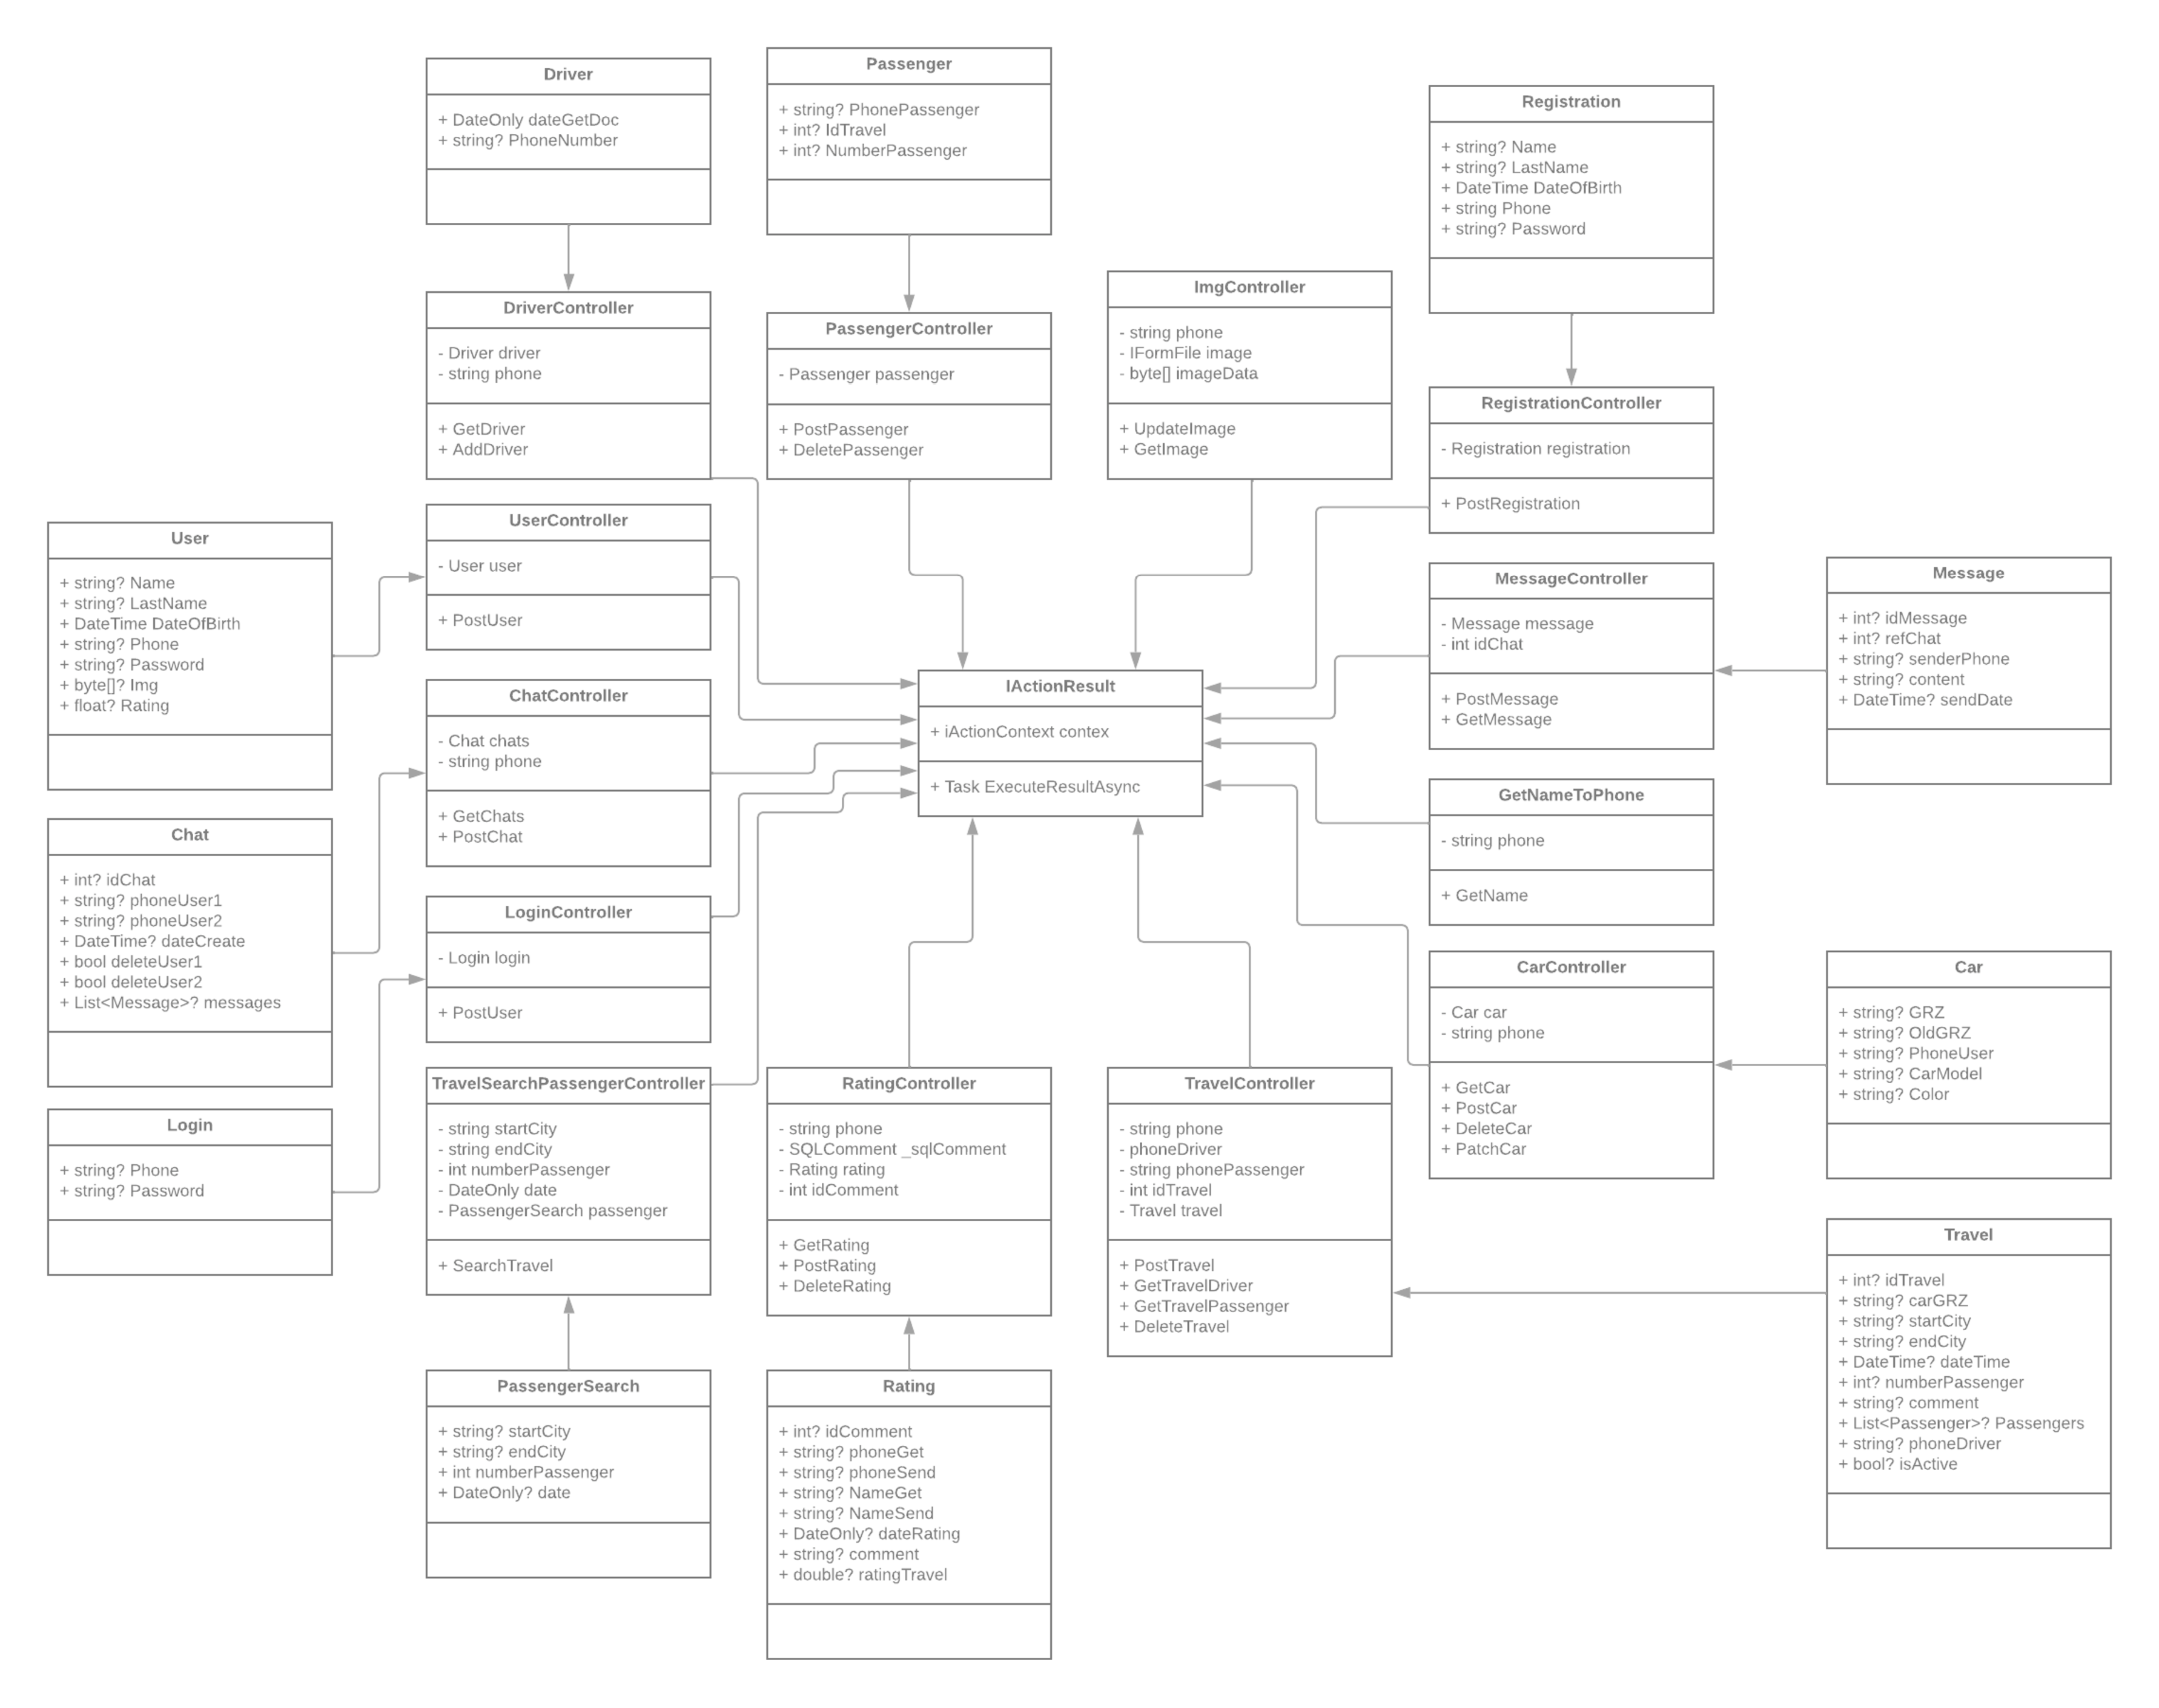
\includegraphics[width=0.9\linewidth]{images/DiagramArch2}
	\caption{Диаграмма классов моделей и контроллеров}
	\label{fig:diagramarch2}
\end{figure}

Driver (Водитель) -- хранит информацию о водителях.

Passenger (Пассажир) -- содержит данные о пассажирах.

User (Пользователь) -- включает основную информацию о пользователях системы.

Chat (Чат) -- содержит информацию о чатах между пользователями.

Login (Логин) -- хранит данные для входа в систему.

Registration (Регистрация) -- содержит информацию для регистрации новых пользователей.

Message (Сообщение) -- представляет сообщения в чатах.

Car (Автомобиль) -- включает данные об автомобилях пользователей.

Travel (Поездка) -- содержит информацию о поездках.

PassengerSearch (Поиск пассажиров) -- используется для поиска пассажиров.

Rating (Рейтинг) -- включает данные о рейтингах пользователей.

DriverController (Контроллер водителей) -- управляет операциями, связанными с водителями.

PassengerController (Контроллер пассажиров) -- обрабатывает операции, связанные с пассажирами.

UserController (Контроллер пользователей) -- управляет действиями, связанными с пользователями.

ChatController (Контроллер чатов) -- управляет взаимодействиями в чатах.

LoginController (Контроллер входа) -- обрабатывает операции входа в систему.

RegistrationController (Контроллер регистрации) -- управляет регистрацией новых пользователей.

MessageController (Контроллер сообщений) -- обрабатывает операции, связанные с сообщениями в чатах.

GetNameToPhone (Контроллер получения имени по телефону) -- предоставляет функциональность получения имени по номеру телефона.

CarController (Контроллер автомобилей) -- управляет данными об автомобилях.

TravelController (Контроллер поездок) -- обрабатывает операции, связанные с поездками.

TravelSearchPassengerController (Контроллер поиска пассажиров для поездок) -- управляет поиском пассажиров для поездок.

RatingController (Контроллер рейтингов) -- управляет данными о рейтингах.


\subsubsection{Архитектура программных классов SQL запросов}

SQLConnectionDb предоставляет стандартные параметры для подключения к базе данных. Этот класс отвечает за установку и хранение параметров подключения, таких как строка подключения и настройки, необходимые для подключения к базе данных.

SqlConnection представляет подключение к базе данных и управляет его состоянием. Это класс от Microsoft, который обеспечивает методы для открытия и закрытия соединения, а также выполнения команд SQL.

DatabaseManager предоставляет асинхронные методы для работы с базой данных. Этот класс управляет открытием и закрытием подключений в асинхронном режиме, что позволяет повысить производительность системы за счет эффективного использования ресурсов и предотвращения блокировок.

На рисунке 3.4 представлена UML-диаграмма классов программной системы, отражающих принцип работы SQL запросов.

\begin{figure}[H]
	\centering
	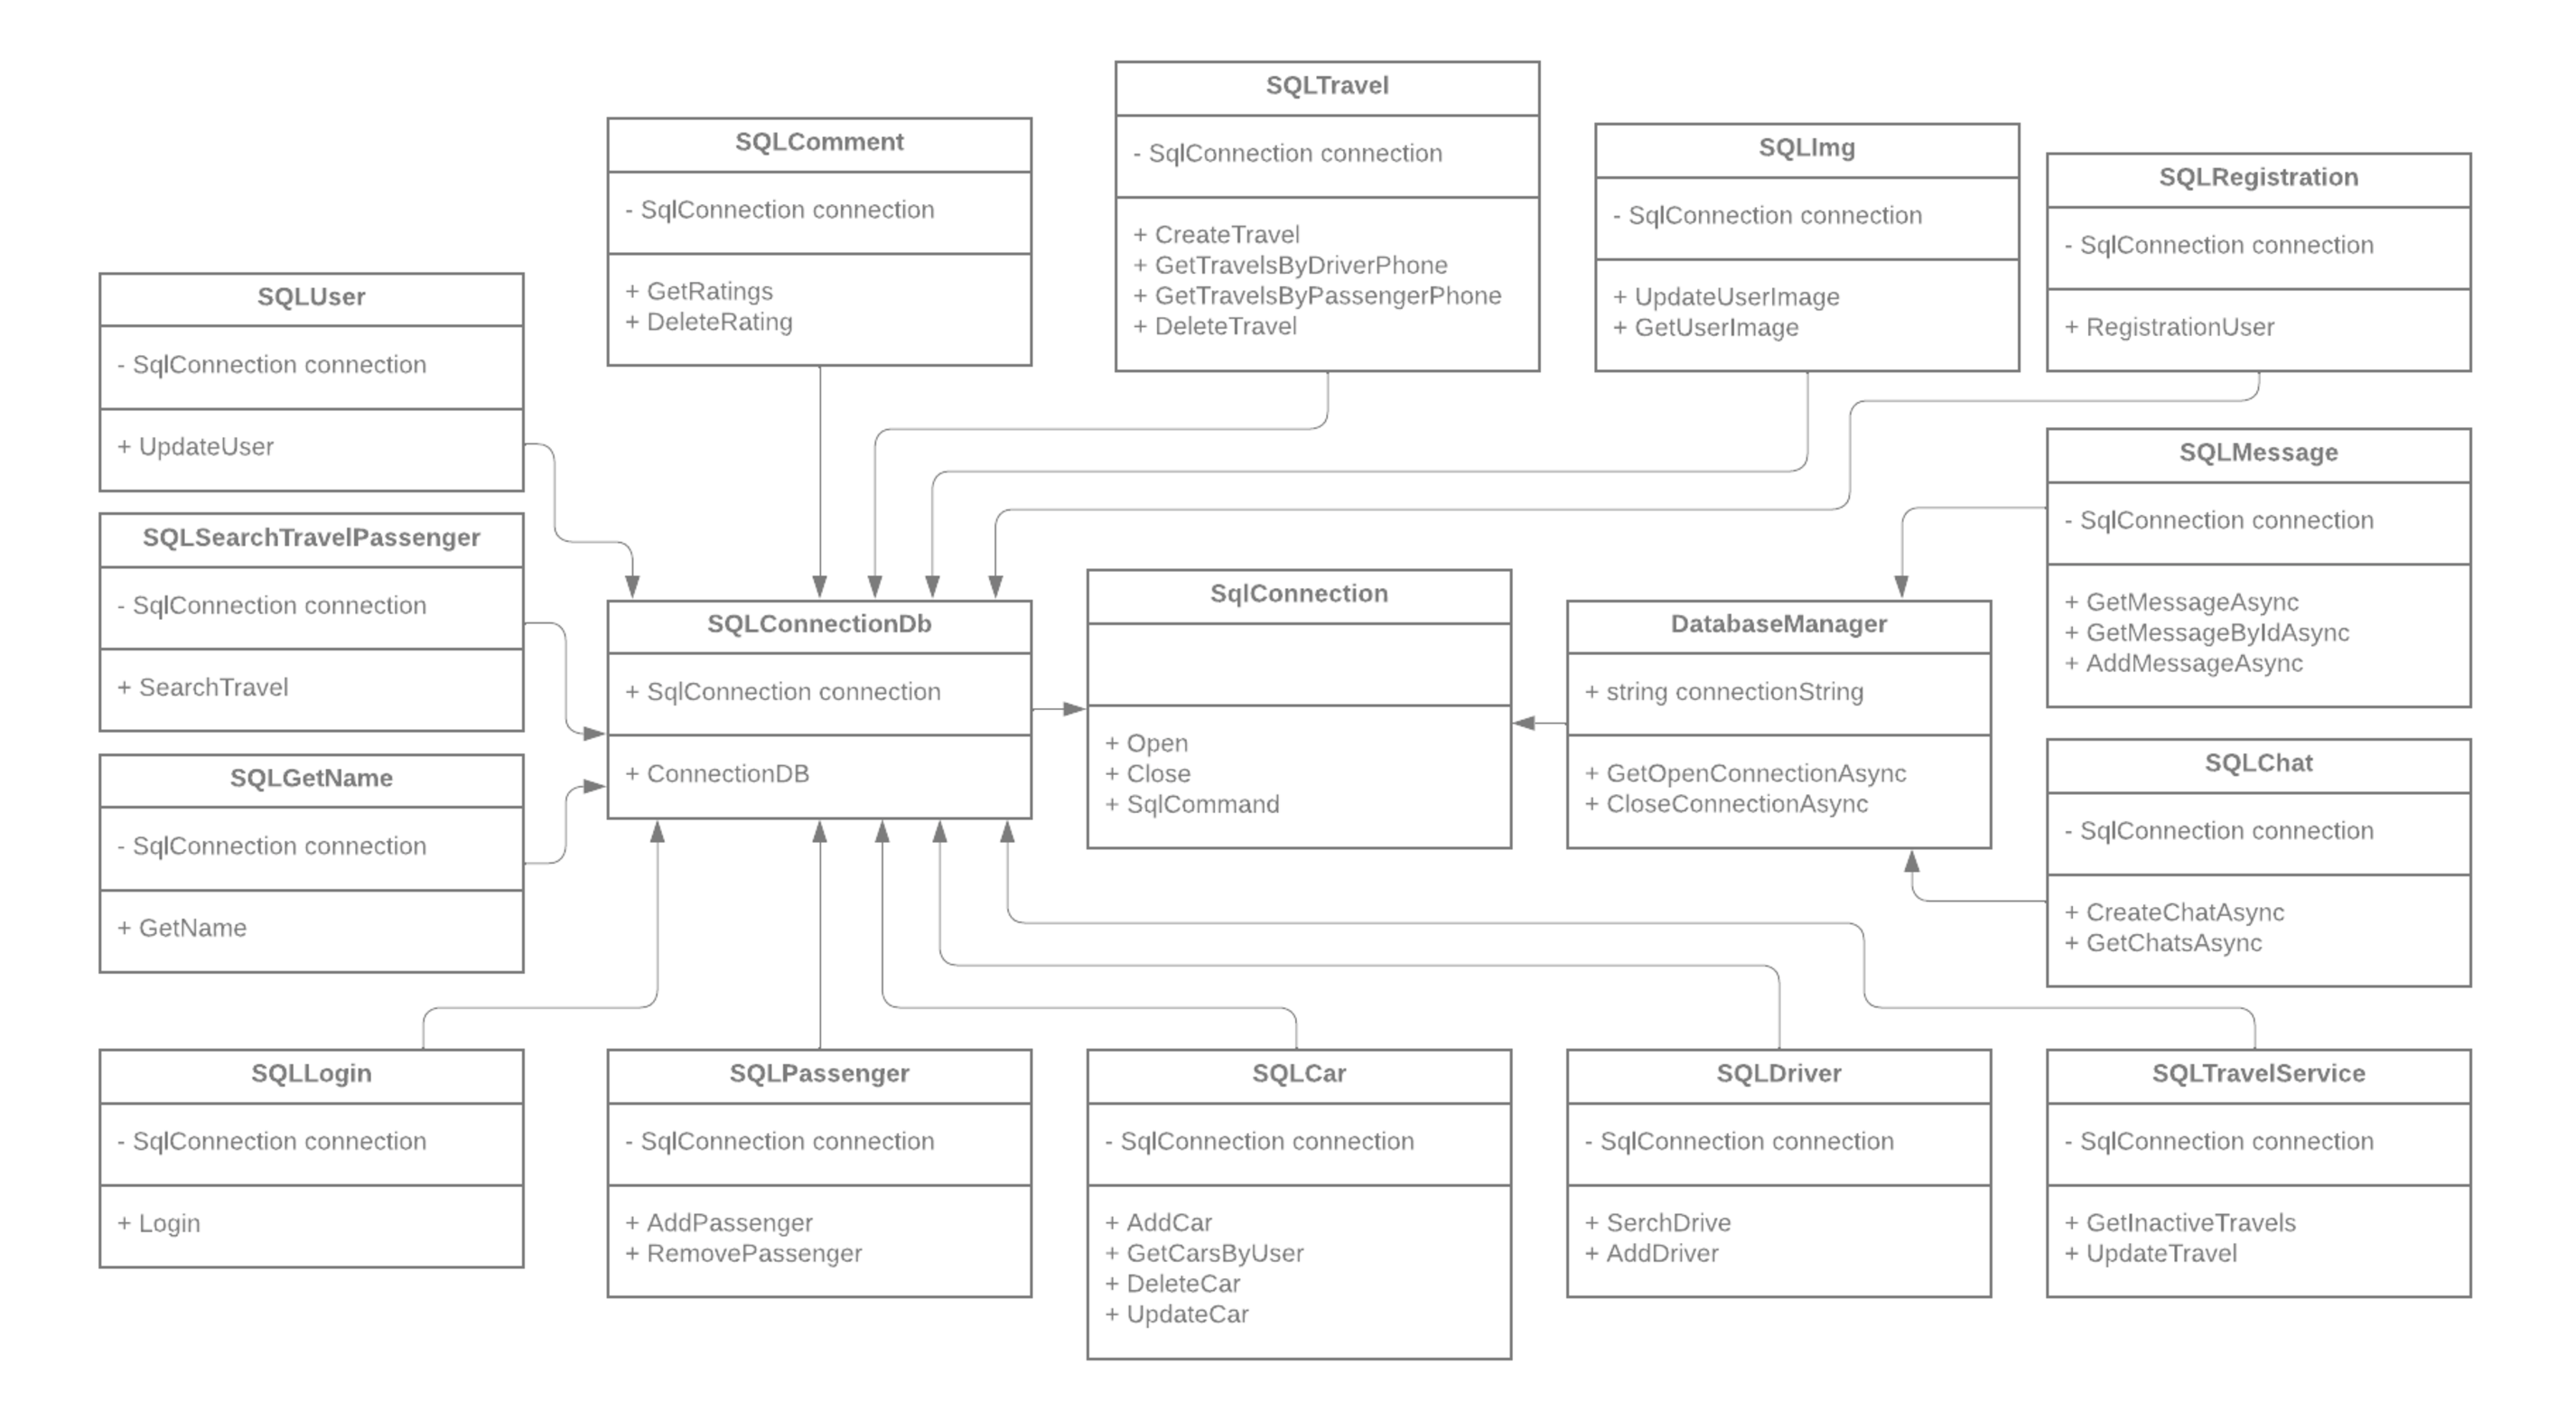
\includegraphics[width=0.9\linewidth]{images/DiagramArch3}
	\caption{Диаграмма классов SQL запросов}
	\label{fig:diagramarch3}
\end{figure}

SQLUser позволяет обновлять информацию о пользователях.

SQLSearchTravelPassenger обеспечивает функциональность поиска пассажиров для поездок.

SQLGetName позволяет получать имя пользователя по номеру телефона.

SQLLogin управляет операциями входа в систему.

SQLPassenger позволяет добавлять и удалять пассажиров.

SQLCar управляет данными об автомобилях, включая добавление, получение, удаление и обновление информации о них.

SQLDriver обеспечивает поиск и добавление водителей.

SQLTravel управляет данными о поездках, включая создание, получение и удаление поездок.

SQLImg позволяет обновлять и получать изображения пользователей.

SQLRegistration управляет регистрацией новых пользователей.

SQLMessage обеспечивает функциональность для работы с сообщениями в чатах, включая их получение и добавление.

SQLChat управляет созданием чатов и получением списка чатов.

SQLTravelService обеспечивает дополнительные сервисы для работы с поездками, такие как получение неактивных поездок и обновление информации о поездках.

SQLComment управляет данными о рейтингах и комментариях, включая их получение и удаление.
